\chapter*{Appendices\label{part:appendices}}
\addcontentsline{toc}{chapter}{Appendices}

\renewcommand{\thesection}{\Alph{section}}
\section{Additional Figures\label{sec:append.figures}}


\begin{figure}[H]
  \centering
  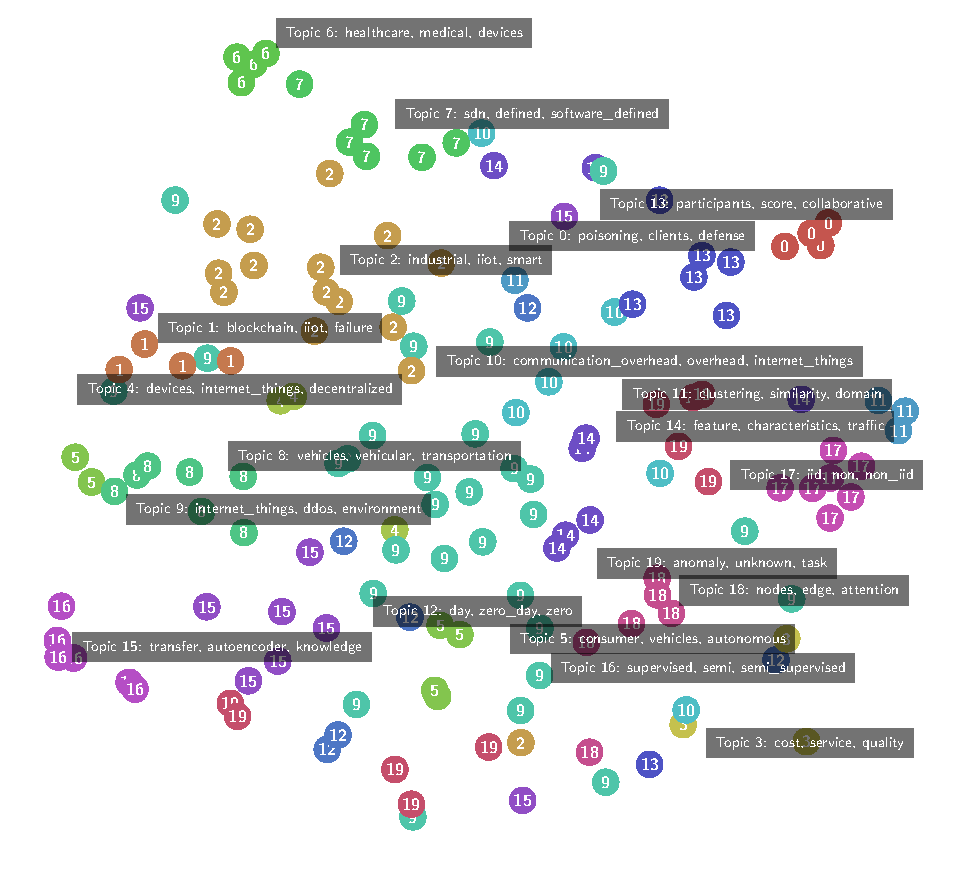
\includegraphics[width=\textwidth]{figures/topic_embedding.pdf}
  \caption{
    Topic embedding of the \gls{fids} literature using a \gls{nmf} model with 20 topics.
    Each point represents a paper, and each are labelled with the topic they are the most associated with.
    \label{fig:append.figure1}
  }
\end{figure}

\newpage
\section{Bibliography for the Automated Literature Review\label{sec:append.biblio}}

{\small
\begin{itemize}
  \item Abbasi M., Taherkordi A., Shahraki A., "FLITC: A Novel Federated Learning-Based Method for IoT Traffic Classification", \textit{in: 8th IEEE International Conference on Smart Computing, SMARTCOMP 2022}, 2022.
  \item Abdel-Basset M., Hawash H., Moustafa N., "Privacy-Preserved Cyberattack Detection in Industrial Edge of Things (IEoT): A Blockchain-Orchestrated Federated Learning Approach", \textit{in: IEEE Transactions on Industrial Informatics}, 2022.
  \item Abosata N., Al-Rubaye S., Inalhan G., "Customised Intrusion Detection for an Industrial IoT Heterogeneous Network Based on Machine Learning Algorithms Called FTL-CID", \textit{in: Sensors}, 2023.
  \item Al-Athba Al-Marri N.A., Ciftler B.S., Abdallah M.M., "Federated Mimic Learning for Privacy Preserving Intrusion Detection", \textit{in: 2020 IEEE International Black Sea Conference on Communications and Networking, BlackSeaCom 2020}, 2020.
  \item Al-Hawawreh M., Hossain M.S., "Federated Learning-assisted Distributed Intrusion Detection Using Mesh Satellite Nets for Autonomous Vehicle Protection", \textit{in: IEEE Transactions on Consumer Electronics}, 2023.
  \item AL-Naday M., Reed M., Dobre V., Toor S., Volckaert B., De Turck F., "Federated deep Q-learning networks for service-based anomaly detection and classification in edge-to-cloud ecosystems", \textit{in: Annales des Telecommunications/Annals of Telecommunications}, 2023.
  \item Al-Naday M., Reed M., Dobre V., Toor S., Volckaert B., De Turck F., "Service-based Federated Deep Reinforcement Learning for Anomaly Detection in Fog Ecosystems", \textit{in: 26th Conference on Innovation in Clouds, Internet and Networks, ICIN 2023}, 2023.
  \item Al-Wesabi F.N., Mengash H.A., Marzouk R., Alruwais N., Allafi R., Alabdan R., Alharbi M., Gupta D., "Pelican Optimization Algorithm with Federated Learning Driven Attack Detection model in Internet of Things environment", \textit{in: Future Generation Computer Systems}, 2023.
  \item Alam M.U., Rahmani R., "FedSepsis: A Federated Multi-Modal Deep Learning-Based Internet of Medical Things Application for Early Detection of Sepsis from Electronic Health Records Using Raspberry Pi and Jetson Nano Devices", \textit{in: Sensors}, 2023.
  \item Alamleh A., Albahri O.S., Alamoodi A.H., Alsatar H.A., Al-Samarraay M.S., Zaidan A.A., Albahri A.S., Zaidan B.B., Qahtan S., Jasim A.N., "Federated Learning for IoMT Applications: A Standardization and Benchmarking Framework of Intrusion Detection Systems", \textit{in: IEEE Journal of Biomedical and Health Informatics}, 2023.
  \item Alazab A., Jan T., Singh S., Khraisat A., "Enhancing Privacy-Preserving Intrusion Detection through Federated Learning", \textit{in: Electronics (Switzerland)}, 2023.
  \item Alazzam M.B., Alassery F., Almulihi A., "Federated Deep Learning Approaches for the Privacy and Security of IoT Systems", \textit{in: Wireless Communications and Mobile Computing}, 2022.
  \item Ali S., Li Q., Yousafzai A., "Blockchain and federated learning-based intrusion detection approaches for edge-enabled industrial IoT networks: a survey", \textit{in: Ad Hoc Networks}, 2024.
  \item Amiri-Zarandi M., Dara R.A., Lin X., "SIDS: A federated learning approach for intrusion detection in IoT using Social Internet of Things", \textit{in: Computer Networks}, 2023.
  \item Aouedi O., Piamrat K., Muller G., Singh K., "Federated Semisupervised Learning for Attack Detection in Industrial Internet of Things", \textit{in: IEEE Transactions on Industrial Informatics}, 2023.
  \item Aouedi O., Piamrat K., Muller G., Singh K., "FLUIDS: Federated Learning with semi-supervised approach for Intrusion Detection System", \textit{in: 19th IEEE Annual Consumer Communications and Networking Conference, CCNC 2022}, 2022.
  \item Arya M., Sastry H., Dewangan B.K., Rahmani M.K.I., Muzaffar A.W., Bhatia S., Bivi M.A., "Intruder Detection in VANET Data Streams Using Federated Learning for Smart City Environments", \textit{in: Electronics (Switzerland)}, 2023.
  \item Ashraf E., Salem H., Areed N.F.F., Abdelhay E.H., Farouk A., "FIDChain: Federated Intrusion Detection System for Blockchain-Enabled IoT Healthcare Applications", \textit{in: Healthcare (Switzerland)}, 2022.
  \item Attanayaka D., Porambage P., Liyanage M., Ylianttila M., "Peer-to-Peer Federated Learning Based Anomaly Detection for Open Radio Access Networks", \textit{in: 2023 IEEE International Conference on Communications, ICC 2023}, 2023.
  \item Attota D.C., Mothukuri V., Parizi R.M., Pouriyeh S., "An Ensemble Multi-View Federated Learning Intrusion Detection for IoT", \textit{in: IEEE Access}, 2021.
  \item Ayed M.A., Talhi C., "Federated Learning for Anomaly-Based Intrusion Detection", \textit{in: 2021 International Symposium on Networks, Computers and Communications, ISNCC 2021}, 2021.
  \item Babbar H., Rani S., "FRHIDS: Federated Learning Recommender Hydrid Intrusion Detection System Model in Software Defined Networking for Consumer Devices", \textit{in: IEEE Transactions on Consumer Electronics}, 2023.
  \item Boudko S., "Federated Learning for Collaborative Cybersecurity of Distributed Healthcare", \textit{in: 21st International Conference on Advances in Mobile Computing and Multimedia Intelligence, MoMM 2023}, 2023.
  \item Cai L., Chen N., Wei Y., Li Y., Chen H., "Cluster-based Federated Learning Framework for Intrusion Detection", \textit{in: 13th IEEE International Symposium on Parallel Architectures, Algorithms and Programming, PAAP 2022}, 2022.
  \item Cetin B., Lazar A., Kim J., Sim A., Wu K., "Federated Wireless Network Intrusion Detection", \textit{in: 2019 IEEE International Conference on Big Data, Big Data 2019}, 2019.
  \item Chandraumakantham O.K., Marappan S., Gajendran S., "Enhancing Intrusion Detection Through Federated Learning With Enhanced Ghost\_BiNet and Homomorphic Encryption", \textit{in: IEEE Access}, 2024.
  \item Chen Z., Lv N., Liu P., Fang Y., Chen K., Pan W., "Intrusion Detection for Wireless Edge Networks Based on Federated Learning", \textit{in: IEEE Access}, 2020.
  \item Chen Y., Zhang J., Yeo C.K., "Network Anomaly Detection Using Federated Deep Autoencoding Gaussian Mixture Model", \textit{in: 2nd International Conference on Machine Learning for Networking, MLN 2019}, 2019.
  \item Chen Y., Zhang J., Yeo C.K., "Privacy-preserving knowledge transfer for intrusion detection with federated deep autoencoding gaussian mixture model", \textit{in: Information Sciences}, 2022.
  \item Cheng Y., Lu J., Lyu B., Zhu S., Niyato D., Kang J., "Federated Transfer Learning with Client Selection for Intrusion Detection in Mobile Edge Computing", \textit{in: IEEE Communications Letters}, 2022.
  \item Cholakoska A., Gjoreski H., Rakovic V., Denkovski D., Kalendar M., Pfitzner B., Arnrich B., "Federated Learning for Network Intrusion Detection in Ambient Assisted Living Environments", \textit{in: IEEE Internet Computing}, 2023.
  \item Cui J., Sun H., Zhong H., Zhang J., Wei L., Bolodurina I., He D., "Collaborative Intrusion Detection System for SDVN: A Fairness Federated Deep Learning Approach", \textit{in: IEEE Transactions on Parallel and Distributed Systems}, 2023.
  \item Cunha Neto H.N., Fernandes N.C., Mattos D.M.F., Hribar J., Dusparic I., "FedSBS: Federated-Learning participant-selection method for Intrusion Detection Systems", \textit{in: Computer Networks}, 2024.
  \item de Caldas Filho F.L., Soares S.C.M., de Oliveira Albuquerque R., da Mata R.Z.A., de Mendonça F.L.L., de Sousa Júnior R.T., Oroski E., "Botnet Detection and Mitigation Model for IoT Networks Using Federated Learning", \textit{in: Sensors}, 2023.
  \item Djaidja T.E.T., Senouci S.M., Brik B., Boualouache A., Ghamri-Doudane Y., "Federated learning for 5G and beyond, a blessing and a curse- an experimental study on intrusion detection systems", \textit{in: Computers and Security}, 2024.
  \item Dong T., Lu J., Qiu H., Qiu M., Fan C., "Towards Fast Network Intrusion Detection based on Efficiency-preserving Federated Learning", \textit{in: 19th IEEE International Symposium on Parallel and Distributed Processing with Applications, 11th IEEE International Conference on Big Data and Cloud Computing, 14th IEEE International Conference on Social Computing and Networking and 11th IEEE International Conference on Sustainable Computing and Communications, ISPA/BDCloud/SocialCom/SustainCom 2021}, 2021.
  \item dos Santos R.R., Viegas E.K., Santin A.O., Tedeschi P., "Federated learning for reliable model updates in network-based intrusion detection", \textit{in: Computers and Security}, 2023.
  \item Driss M., Almomani I., e Huma Z., Ahmad J., "A federated learning framework for cyberattack detection in vehicular sensor networks", \textit{in: Complex and Intelligent Systems}, 2022.
  \item Duy P.T., Hung T.V., Ha N.H., Hoang H.D., Pham V.H., "Federated learning-based intrusion detection in SDN-enabled IIoT networks", \textit{in: 8th NAFOSTED Conference on Information and Computer Science, NICS 2021}, 2021.
  \item Fan Y., Li Y., Zhan M., Cui H., Zhang Y., "IoTDefender: A Federated Transfer Learning Intrusion Detection Framework for 5G IoT", \textit{in: 14th IEEE International Conference on Big Data Science and Engineering, BigDataSE 2020}, 2020.
  \item Fan M., Ji K., Zhang Z., Yu H., Sun G., "Lightweight Privacy and Security Computing for Blockchained Federated Learning in IoT", \textit{in: IEEE Internet of Things Journal}, 2023.
  \item Fan J., Wu K., Tang G., Zhou Y., Huang S., "Taking Advantage of the Mistakes: Rethinking Clustered Federated Learning for IoT Anomaly Detection", \textit{in: IEEE Transactions on Parallel and Distributed Systems}, 2024.
  \item Friha O., Ferrag M.A., Benbouzid M., Berghout T., Kantarci B., Choo K.K.R., "2DF-IDS: Decentralized and differentially private federated learning-based intrusion detection system for industrial IoT", \textit{in: Computers and Security}, 2023.
  \item Friha O., Nafaa M., Ferrag M.A., Shu L., Maglaras L., Choo K.K.R., "FELIDS: Federated learning-based intrusion detection system for agricultural Internet of Things", \textit{in: Journal of Parallel and Distributed Computing}, 2022.
  \item Hajj S., Ginhac D., Azar J., Guyeux C., Makhoul A., Bou Abdo J., Demerjian J., "Cross-Layer Federated Learning for Lightweight IoT Intrusion Detection Systems", \textit{in: Sensors}, 2023.
  \item Hamdi N., "Federated learning-based intrusion detection system for Internet of Things", \textit{in: International Journal of Information Security}, 2023.
  \item Han W., Peng J., Yu J., Kang J., Lu J., Niyato D., "Heterogeneous Data-Aware Federated Learning for Intrusion Detection Systems via Meta-sampling in Artificial Intelligence of Things", \textit{in: IEEE Internet of Things Journal}, 2023.
  \item Hbaieb A., Ayed S., Chaari L., "Federated learning based IDS approach for the IoV", \textit{in: 17th International Conference on Availability, Reliability and Security, ARES 2022}, 2022.
  \item He S., Du C., Hossain M.S., "6G-enabled Consumer Electronics Device Intrusion Detection with Federated Meta-Learning and Digital Twins in a Meta-Verse Environment", \textit{in: IEEE Transactions on Consumer Electronics}, 2023.
  \item He X., Chen Q., Tang L., Wang W., Liu T., "CGAN-Based Collaborative Intrusion Detection for UAV Networks: A Blockchain-Empowered Distributed Federated Learning Approach", \textit{in: IEEE Internet of Things Journal}, 2023.
  \item He X., Chen Q., Tang L., Wang W., Liu T., Li L., Liu Q., Luo J., "Federated Continuous Learning Based on Stacked Broad Learning System Assisted by Digital Twin Networks: An Incremental Learning Approach for Intrusion Detection in UAV Networks", \textit{in: IEEE Internet of Things Journal}, 2023.
  \item Hei X., Yin X., Wang Y., Ren J., Zhu L., "A trusted feature aggregator federated learning for distributed malicious attack detection", \textit{in: Computers and Security}, 2020.
  \item Houda Z.A.E., Moudoud H., Brik B., Khoukhi L., "Blockchain-Enabled Federated Learning for Enhanced Collaborative Intrusion Detection in Vehicular Edge Computing", \textit{in: IEEE Transactions on Intelligent Transportation Systems}, 2024.
  \item Hu Y., Fu X., Zeng W., "Distributed Fire Detection and Localization Model Using Federated Learning", \textit{in: Mathematics}, 2023.
  \item Hu Y., Wu J., Li G., Li J., Cheng J., "Privacy-preserving Few-shot Traffic Detection against Advanced Persistent Threats via Federated Meta Learning", \textit{in: IEEE Transactions on Network Science and Engineering}, 2023.
  \item Huang X., Liu J., Lai Y., Mao B., Lyu H., "EEFED: Personalized Federated Learning of Execution\&Evaluation Dual Network for CPS Intrusion Detection", \textit{in: IEEE Transactions on Information Forensics and Security}, 2023.
  \item Idrissi M.J., Alami H., El Mekki A., Berrada I., El Mahdaouy A., Oualil S., Yartaoui Z., "Fed-ANIDS: Federated learning for anomaly-based network intrusion detection systems", \textit{in: Expert Systems with Applications}, 2023.
  \item Nagaradjane P., Angin P., Balasubramanian P., Ioannou I., Vassiliou V., Kavitha K.J., Murugan P., "GEMLIDS-MIOT: A Green Effective Machine Learning Intrusion Detection System based on Federated Learning for Medical IoT network security hardening", \textit{in: Computer Communications}, 2024.
  \item Islam M.M., Islam A.B.M.A.A., "Disparity-Aware Federated Learning for Intrusion Detection Systems in Imbalanced Non-IID Settings", \textit{in: 10th International Conference on Networking Systems and Security, NSysS 2023}, 2023.
  \item Jahromi A.N., Schulich H.K., Dehghantanha A., "Deep Federated Learning-Based Cyber-Attack Detection in Industrial Control Systems", \textit{in: 18th International Conference on Privacy, Security and Trust, PST 2021}, 2021.
  \item Jahromi A.N., Karimipour H., Dehghantanha A., "An ensemble deep federated learning cyber-threat hunting model for Industrial Internet of Things", \textit{in: Computer Communications}, 2023.
  \item Ji X., Zhang H., Ma X., "A Novel Method of Intrusion Detection Based on Federated Transfer Learning and Convolutional Neural Network", \textit{in: 10th IEEE Joint International Information Technology and Artificial Intelligence Conference, ITAIC 2022}, 2022.
  \item Jiang T., Shen G., Guo C., Cui Y., Xie B., "BFLS: Blockchain and Federated Learning for sharing threat detection models as Cyber Threat Intelligence", \textit{in: Computer Networks}, 2023.
  \item Jin D., Chen S., He H., Jiang X., Cheng S., Yang J., "Federated Incremental Learning based Evolvable Intrusion Detection System for Zero-Day Attacks", \textit{in: IEEE Network}, 2023.
  \item Jin Z., Wu X., Zhou J., Li B., Duan C., "FL-IIDS: A novel federated learning-based incremental intrusion detection system", \textit{in: Future Generation Computer Systems}, 2024.
  \item Khan I.A., Pi D., Hussain Y., Soliman H., Abbas M.Z., Zia U., "Federated-SRUs: A Federated-Simple-Recurrent-Units-Based IDS for Accurate Detection of Cyber Attacks Against IoT-Augmented Industrial Control Systems", \textit{in: IEEE Internet of Things Journal}, 2023.
  \item Kim S., Cai H., Hua C., Gu P., Xu W., Park J., "Collaborative Anomaly Detection for Internet of Things based on Federated Learning", \textit{in: 2020 IEEE/CIC International Conference on Communications in China, ICCC 2020}, 2020.
  \item Kollu V.N., Janarthanan V., Karupusamy M., Ramachandran M., "Cloud-Based Smart Contract Analysis in FinTech Using IoT-Integrated Federated Learning in Intrusion Detection", \textit{in: Data}, 2023.
  \item Kristianto E., Lin P.C., Hwang R.H., "Misbehavior detection system with semi-supervised federated learning", \textit{in: Vehicular Communications}, 2023.
  \item Kumar R., Kumar P., Tripathi R., Gupta G.P., Garg S., Hassan M.M., "A distributed intrusion detection system to detect DDoS attacks in blockchain-enabled IoT network", \textit{in: Journal of Parallel and Distributed Computing}, 2022.
  \item Lai Y.C., Lin J.Y., Lin Y.D., Hwang R.H., Lin P.C., Wu H.K., Chen C.K., "Two-phase Defense Against Poisoning Attacks on Federated Learning-based Intrusion Detection", \textit{in: Computers and Security}, 2023.
  \item Lalouani W., Younis M., "Robust Distributed Intrusion Detection System for Edge of Things", \textit{in: 2021 IEEE Global Communications Conference, GLOBECOM 2021}, 2021.
  \item Lazzarini R., Tianfield H., Charissis V., "Federated Learning for IoT Intrusion Detection", \textit{in: AI (Switzerland)}, 2023.
  \item Li K., Zhou H., Tu Z., Liu F., Zhang H., "Blockchain Empowered Federated Learning for Distributed Network Security Behaviour Knowledge Base in 6G", \textit{in: Security and Communication Networks}, 2022.
  \item Li B., Wu Y., Song J., Li T., Zhao L., Lu R., "DeepFed: Federated Deep Learning for Intrusion Detection in Industrial Cyber-Physical Systems", \textit{in: IEEE Transactions on Industrial Informatics}, 2021.
  \item Li K., Zhou H., Tu Z., Wang W., Zhang H., "Distributed Network Intrusion Detection System in Satellite-Terrestrial Integrated Networks Using Federated Learning", \textit{in: IEEE Access}, 2020.
  \item Li J., Tong X., Cheng L., Liu J., "An Efficient Federated Learning System for Network Intrusion Detection", \textit{in: IEEE Systems Journal}, 2023.
  \item Li B., Ma S., Yang J., Deng R., Choo K.K.R., "Federated Anomaly Detection on System Logs for the Internet of Things: A Customizable and Communication-Efficient Approach", \textit{in: IEEE Transactions on Network and Service Management}, 2022.
  \item Lian Z., Su C., "Decentralized Federated Learning for Internet of Things Anomaly Detection", \textit{in: 17th ACM ASIA Conference on Computer and Communications Security 2022, ASIA CCS 2022}, 2022.
  \item Liang H., Liu D., Zeng X., Ye C., "An Intrusion Detection Method for Advanced Metering Infrastructure System Based on Federated Learning", \textit{in: Journal of Modern Power Systems and Clean Energy}, 2023.
  \item Liu Z., Guo C., Yin X., Liu D., "An Asynchronous Federated Learning Arbitration Model for Low-Rate DDoS Attack Detection", \textit{in: IEEE Access}, 2023.
  \item Liu H., Zhou X., Pu G., Zhang S., Zhang P., Shao X., Zhang Y., "Blockchain and Federated Learning for Collaborative Intrusion Detection in Vehicular Edge Computing", \textit{in: IEEE Transactions on Vehicular Technology}, 2021.
  \item Liu S., Yu Y., Zong Y., Yeoh P.L., Guo L., Vucetic B., Li Y., Duong T.Q., "Delay and Energy-Efficient Asynchronous Federated Learning for Intrusion Detection in Heterogeneous Industrial Internet of Things", \textit{in: IEEE Internet of Things Journal}, 2023.
  \item Liu Y., Wu G., Zhang W., Li J., "Federated Learning-Based Intrusion Detection on Non-IID Data", \textit{in: 22nd International Conference on Algorithms and Architectures for Parallel Processing, ICA3PP 2022}, 2022.
  \item Liu W., Xu X., Wu L., Qi L., Jolfaei A., Ding W., Khosravi M.R., "Intrusion Detection for Maritime Transportation Systems with Batch Federated Aggregation", \textit{in: IEEE Transactions on Intelligent Transportation Systems}, 2023.
  \item Lv P., Xu J., Wu X., Xie L., Li T., "Misbehavior Detection in Vehicular Ad Hoc Networks Based on Privacy-Preserving Federated Learning and Blockchain", \textit{in: IEEE Transactions on Network and Service Management}, 2022.
  \item Madala C.J.S., Yadav G.H.K., Sivakumar S., Nithya R., Manjunatha K.M., Deivakani M., "Federated Learning Approach for Tracking Malicious Activities in Cyber-Physical Systems", \textit{in: 2022 International Conference on Edge Computing and Applications, ICECAA 2022}, 2022.
  \item Mahmoodi A.B.Z., Sheikhi S., Peltonen E., Kostakos P., "Autonomous Federated Learning for Distributed Intrusion Detection Systems in Public Networks", \textit{in: IEEE Access}, 2023.
  \item Manyadza T.J., Du H., Wang S., Yang W., Chen C., Tian F., "FL-finder: Detecting Unknown Network Anomaly in Federated Learning", \textit{in: 5th IEEE International Conference on Artificial Intelligence and Big Data, ICAIBD 2022}, 2022.
  \item Marfo W., Tosh D.K., Moore S.V., "Network Anomaly Detection Using Federated Learning", \textit{in: 2022 IEEE Military Communications Conference, MILCOM 2022}, 2022.
  \item Mármol Campos E., Hernandez-Ramos J.L., González Vidal A., Skarmeta A., Baldini G., "Misbehavior detection in intelligent transportation systems based on federated learning", \textit{in: Internet of Things (Netherlands)}, 2024.
  \item Merzouk M.A., Cuppens F., Boulahia-Cuppens N., Yaich R., "Parameterizing poisoning attacks in federated learning-based intrusion detection", \textit{in: 18th International Conference on Availability, Reliability and Security, ARES 2023}, 2023.
  \item Mokry L., Slife P., Bishop P., Quiroz J., Guzzi C., Crainiceanu A., Needham D., Chen Z., "Efficient and Privacy-Preserving Collaborative Intrusion Detection Using Additive Secret Sharing and Differential Privacy", \textit{in: 2021 IEEE International Conference on Big Data, Big Data 2021}, 2021.
  \item Moustafa N., Khan I.A., Pi D., Hassanin M., Ormrod D., Slay J., Razzak I., "DFSat: Deep Federated Learning for Identifying Cyber Threats in IoT-based Satellite Networks", \textit{in: IEEE Transactions on Industrial Informatics}, 2022.
  \item Naeem F., Ali M., Kaddoum G., "Federated-Learning-Empowered Semi-Supervised Active Learning Framework for Intrusion Detection in ZSM", \textit{in: IEEE Communications Magazine}, 2023.
  \item Neto E.C.P., Dadkhah S., Ghorbani A.A., "Collaborative DDoS Detection in Distributed Multi-Tenant IoT using Federated Learning", \textit{in: 19th Annual International Conference on Privacy, Security and Trust, PST 2022}, 2022.
  \item Neto H.N.C., Mattos D.M.F., Fernande N.C., Dusparic I., "FedSA: Accelerating Intrusion Detection in Collaborative Environments with Federated Simulated Annealing", \textit{in: 8th IEEE International Conference on Network Softwarization, NetSoft 2022}, 2022.
  \item Nguyen T.D., Miettinen M., Fereidooni H., Sadeghi A.R., Marchal S., Asokan N., "DÏoT: A federated self-learning anomaly detection system for IoT", \textit{in: 39th IEEE International Conference on Distributed Computing Systems, ICDCS 2019}, 2019.
  \item Novikova E., Doynikova E., Golubev S., "Federated Learning for Intrusion Detection in the Critical Infrastructures: Vertically Partitioned Data Use Case", \textit{in: Algorithms}, 2022.
  \item Oh H., Yu J., Kim N., Kim D., Lee J., Yang J., "A federated binarized neural network model for constrained devices in IoT healthcare services", \textit{in: 4th International Conference on Artificial Intelligence in Information and Communication, ICAIIC 2022}, 2022.
  \item Otoum S., Guizani N., Mouftah H., "On the Feasibility of Split Learning, Transfer Learning and Federated Learning for Preserving Security in ITS Systems", \textit{in: IEEE Transactions on Intelligent Transportation Systems}, 2023.
  \item Otoum Y., Wan Y., Nayak A., "Federated Transfer Learning-Based IDS for the Internet of Medical Things (IoMT)", \textit{in: 2021 IEEE Globecom Workshops, GC Wkshps 2021}, 2021.
  \item Pahl M., Aubet F., "All Eyes on You: Distributed Multi-Dimensional IoT Microservice Anomaly Detection", \textit{in: 14th International Conference on Network and Service Management, CNSM 2018 and Workshops, 1st International Workshop on High-Precision Networks Operations and Control, HiPNet 2018 and 1st Workshop on Segment Routing and Service Function Chaining, SR+SFC 2018}, 2018.
  \item Panagoda D., Malinda C., Wijetunga C., Rupasinghe L., Bandara B., Liyanapathirana C., "Application of Federated Learning in Health Care Sector for Malware Detection and Mitigation Using Software Defined Networking Approach", \textit{in: 2nd Asian Conference on Innovation in Technology, ASIANCON 2022}, 2022.
  \item Pei J., Li J., Zhong K., Jan M.A., "Personalized federated learning framework for network traffic anomaly detection", \textit{in: Computer Networks}, 2022.
  \item Phan T.V., Nguyen T.G., "FEAR: Federated Cyber-Attack Reaction in Distributed Software-Defined Networks with Deep Q-Network", \textit{in: 21st Annual Wireless Telecommunications Symposium, WTS 2022}, 2022.
  \item Popoola S.I., Gui G., Adebisi B., Hammoudeh M., Gacanin H., "Federated Deep Learning for Collaborative Intrusion Detection in Heterogeneous Networks", \textit{in: 94th IEEE Vehicular Technology Conference, VTC 2021-Fall}, 2021.
  \item Popoola S.I., Adebisi B., Jogunola O., Ande R., Gui G., Hammoudeh M., "Federated Deep Learning for Zero-Day Botnet Attack Detection in IoT-Edge Devices", \textit{in: IEEE Internet of Things Journal}, 2022.
  \item Popoola S.I., Jogunola O., Imoize A.L., Hammoudeh M., Adebisi B., Aibinu A.M., "Federated Deep Learning for Intrusion Detection in Consumer-Centric Internet of Things", \textit{in: IEEE Transactions on Consumer Electronics}, 2023.
  \item Pourahmadi V., Salahuddin M.A., Boutaba R., Alameddine H.A., "Spotting Anomalies at the Edge: Outlier Exposure-Based Cross-Silo Federated Learning for DDoS Detection", \textit{in: IEEE Transactions on Dependable and Secure Computing}, 2023.
  \item Preuveneers D., Rimmer V., Tsingenopoulos I., Spooren J., Joosen W., Ilie-Zudor E., "Chained anomaly detection models for federated learning: An intrusion detection case study", \textit{in: Applied Sciences (Switzerland)}, 2018.
  \item Qin Y., Kondo M., "Federated Learning-Based Network Intrusion Detection with a Feature Selection Approach", \textit{in: 3rd International Conference on Electrical, Communication and Computer Engineering, ICECCE 2021}, 2021.
  \item Qin Q., Poularakis K., Tassiulas L., Leung K.K., "Line-Speed and Scalable Intrusion Detection at the Network Edge via Federated Learning", \textit{in: 2020 IFIP Networking Conference and Workshops, Networking 2020}, 2020.
  \item Quyen N.H., Duy P.T., Vy N.C., Hien D.T.T., Pham V.H., "Federated Intrusion Detection on Non-IID Data for IIoT Networks Using Generative Adversarial Networks and Reinforcement Learning", \textit{in: 17th International Conference on Information Security Practice and Experience, ISPEC 2022}, 2022.
  \item Rahman S.A., Tout H., Talhi C., Mourad A., "Internet of Things intrusion Detection: Centralized, On-Device, or Federated Learning?", \textit{in: IEEE Network}, 2020.
  \item Rashid M.M., Khan S.U., Eusufzai F., Redwan M.A., Sabuj S.R., Elsharief M., "A Federated Learning-Based Approach for Improving Intrusion Detection in Industrial Internet of Things Networks", \textit{in: Network}, 2023.
  \item Rathore S., Wook Kwon B., Park J.H., "BlockSecIoTNet: Blockchain-based decentralized security architecture for IoT network", \textit{in: Journal of Network and Computer Applications}, 2019.
  \item Senevirathna T.T., Liyanage M., Porambage P., Ylianttila M., Rumesh Y., "Comprehensive Analysis Over Centralized and Federated Learning-Based Anomaly Detection in Networks with Explainable AI (XAI)", \textit{in: 2023 IEEE International Conference on Communications, ICC 2023}, 2023.
  \item Shafee A., Baza M., Fouda M.M., Mahmoud M., Talbert D.A., Nabil M., "Mimic Learning to Generate a Shareable Network Intrusion Detection Model", \textit{in: 17th IEEE Annual Consumer Communications and Networking Conference, CCNC 2020}, 2020.
  \item Shan Y., Yao Y., Zhao T., Zhou X., Wang L., Hu B., "CFL-IDS: An Effective Clustered Federated Learning Framework for Industrial Internet of Things Intrusion Detection", \textit{in: IEEE Internet of Things Journal}, 2024.
  \item Sharma P., Sharma S.K., Dani D., "Edge-assisted federated learning for anomaly detection in diverse IoT network", \textit{in: International Journal of Information Technology (Singapore)}, 2024.
  \item Shi J., Yan Y., Li S., Ge B., Liu Y., "Data privacy security guaranteed network intrusion detection system based on federated learning", \textit{in: 2021 IEEE Conference on Computer Communications Workshops, INFOCOM WKSHPS 2021}, 2021.
  \item Singh P., Hedabou M., Kaur A., Gaba G.S., Gurtov A., "Dew-Cloud-Based Hierarchical Federated Learning for Intrusion Detection in IoMT", \textit{in: IEEE Journal of Biomedical and Health Informatics}, 2023.
  \item Su D., Qu Z., "Detection DDoS of Attacks Based on Federated Learning with Digital Twin Network", \textit{in: 15th International Conference on Knowledge Science, Engineering and Management, KSEM 2022}, 2022.
  \item Sun Y., Esaki H., Ochiai H., "Adaptive Intrusion Detection in the Networking of Large-Scale LANs with Segmented Federated Learning", \textit{in: IEEE Open Journal of the Communications Society}, 2021.
  \item Sun Y., Ochiai H., Esaki H., "Intrusion Detection with Segmented Federated Learning for Large-Scale Multiple LANs", \textit{in: 2020 International Joint Conference on Neural Networks, IJCNN 2020}, 2020.
  \item Tabassum A., Lebda W., Mohamed A., Guizani M., Erbad A., "FEDGAN-IDS: Privacy-preserving IDS using GAN and Federated Learning", \textit{in: Computer Communications}, 2022.
  \item Tahir B., Tariq M., Jolfaei A., "Experience-Driven Attack Design and Federated-Learning-Based Intrusion Detection in Industry 4.0", \textit{in: IEEE Transactions on Industrial Informatics}, 2022.
  \item Tang Z., Hu H., Xu C., "A federated learning method for network intrusion detection", \textit{in: Concurrency and Computation: Practice and Experience}, 2022.
  \item Thein T.T., Shiraishi Y., Morii M., "Personalized federated learning-based intrusion detection system: Poisoning attack and defense", \textit{in: Future Generation Computer Systems}, 2024.
  \item Thi H.T., Hoang Son N.D., Duv P.T., Van Pham H., "Federated Learning-Based Cyber Threat Hunting for APT Attack Detection in SDN-Enabled Networks", \textit{in: 21st International Symposium on Communications and Information Technologies, ISCIT 2022}, 2022.
  \item Truong H.T., Le Q.A., Nguyen D.M., Le C.T., Nguyen H.X., Nguyen H.T., Ta B.P., Do H.T., Tran K.P., "Light-weight federated learning-based anomaly detection for time-series data in industrial control systems", \textit{in: Computers in Industry}, 2022.
  \item Vadigi S., Mohanty D., Bera P., Sethi K., Das S.P., "Federated reinforcement learning based intrusion detection system using dynamic attention mechanism", \textit{in: Journal of Information Security and Applications}, 2023.
  \item Vaiyapuri T., Sbai Z., Al-Helal M., Algamdi S., John R., alkhayyat A., Gupta D., "Metaheuristics with federated learning enabled intrusion detection system in Internet of Things environment", \textit{in: Expert Systems}, 2022.
  \item Verma P., Breslin J.G., O’Shea D., "FLDID: Federated Learning Enabled Deep Intrusion Detection in Smart Manufacturing Industries", \textit{in: Sensors}, 2022.
  \item Wang K., Li J., Wu W., "An Efficient Intrusion Detection Method Based on Federated Transfer Learning and an Extreme Learning Machine with Privacy Preservation", \textit{in: Security and Communication Networks}, 2022.
  \item Wang N., Chen Y., Hu Y., Lou W., Hou Y.T., "FeCo: Boosting Intrusion Detection Capability in IoT Networks via Contrastive Learning", \textit{in: 41st IEEE Conference on Computer Communications, INFOCOM 2022}, 2022.
  \item Wang X., Wang Y., Javaheri Z., Moghadamnejad N., Almutairi L., Younes O.S., "Federated deep learning for anomaly detection in the internet of things", \textit{in: Computers and Electrical Engineering}, 2023.
  \item Wang Z.X., Wang P., Sun Z.X., "SDN traffic anomaly detection method based on convolutional autoencoder and federated learning", \textit{in: 2022 IEEE Global Communications Conference, GLOBECOM 2022}, 2022.
  \item Wasielewska K., Camacho J., Soukup D., Čejka T., "Evaluation of the Limit of Detection in Network Dataset Quality Assessment with PerQoDA", \textit{in: Workshops on SoGood, NFMCP, XKDD, UMOD, ITEM, MIDAS, MLCS, MLBEM, PharML, DALS, IoT-PdM 2022, held in conjunction with the 21st Joint European Conference on Machine Learning and Principles and Practice of Knowledge Discovery in Databases, ECML PKDD 2022}, 2022.
  \item Xia Q., Peng T., Dong S., "An Abnormal Traffic Detection Method for IoT Devices Based on Federated Learning and Depthwise Separable Convolutional Neural Networks", \textit{in: 2022 IEEE International Performance, Computing, and Communications Conference, IPCCC 2022}, 2022.
  \item Xing L., Wang K., Wu H., Ma H., Zhang X., "FL-MAAE: An Intrusion Detection Method for the Internet of Vehicles Based on Federated Learning and Memory-Augmented Autoencoder", \textit{in: Electronics (Switzerland)}, 2023.
  \item Yadav K., Gupta B.B., Hsu C.H., Chui K.T., "Unsupervised Federated Learning based IoT Intrusion Detection", \textit{in: 10th IEEE Global Conference on Consumer Electronics, GCCE 2021}, 2021.
  \item Yang R., He H., Qu Y., Zhang W., Wang Y., "Dependable federated learning for IoT intrusion detection against poisoning attacks", \textit{in: Computers and Security}, 2023.
  \item Yuan S., Li H., Zhang R., Hao M., Li Y., Lu R., "Towards Lightweight and Efficient Distributed Intrusion Detection Framework", \textit{in: 2021 IEEE Global Communications Conference, GLOBECOM 2021}, 2021.
  \item Zaabar B., Cheikhrouhou O., Abid M., "Intrusion Detection System for IoMT through Blockchain-based Federated Learning", \textit{in: 15th IEEE International Conference on Security of Information and Networks, SIN 2022}, 2022.
  \item Zakariyya I., Kalutarage H., Al-Kadri M.O., "Resource Efficient Federated Deep Learning for IoT Security Monitoring", \textit{in: 5th International Workshop on Attacks and Defenses for Internet-of-Things, ADIoT 2022, held in conjunction with 27th European Symposium on Research in Computer Security, ESORICS 2022}, 2022.
  \item Zhang W., Yu Q., Li Z., Lu Q., Liu Y., Lo S.K., Chen S., Xu X., Zhu L., "Blockchain-based federated learning for device failure detection in industrial iot", \textit{in: IEEE Internet of Things Journal}, 2021.
  \item Zhang Q., Wang Y., Wei T., Wen J., Chen J., Qiu X., "IoT Intrusion Detection Based on Personalized Federated Learning", \textit{in: 24th Asia-Pacific Network Operations and Management Symposium, APNOMS 2023}, 2023.
  \item Zhang Z., Zhang Y., Guo D., Yao L., Li Z., "SecFedNIDS: Robust defense for poisoning attack against federated learning-based network intrusion detection system", \textit{in: Future Generation Computer Systems}, 2022.
  \item Zhao Y., Chen J., Teng J., Wu D., Yu S., "Multi-task network anomaly detection using federated learning", \textit{in: 10th International Symposium on Information and Communication Technology, SoICT 2019}, 2019.
  \item Zhao R., Wang Y., Xue Z., Ohtsuki T., Adebisi B., Gui G., "Semisupervised Federated-Learning-Based Intrusion Detection Method for Internet of Things", \textit{in: IEEE Internet of Things Journal}, 2023.
  \item Zhu M.y., Lv N., Chen Z., Chen K.f., Zhong Y., "Attention-based federated incremental learning for traffic classification in the Internet of Things", \textit{in: Computer Communications}, 2022.
\end{itemize}
}

\newpage
\selectlanguage{french}
\section{Résumé en français de la thèse\label{sec:french}}

La sécurisation des systèmes d'information se complexifie à mesure que ceux-ci gagnent en taille et en complexité. 
Parce que la sécurité par conception est bien souvent inapplicable, les différentes agences gouvernementales recommandent des mesures de sécurité complémentaires, telles que le déploiement de solutions de détection.
Les systèmes de détection d'intrusions (IDS en anglais) bénéficient grandement des dernières avances en apprentissage machine (ML), mais se heurtent aussi aux limitations de ces derniers.
En particulier, l'important coût humain et financier de la génération de données étiquetées pour entraîner des algorithmes d'apprentissage rend leur déploiement difficile pour les organisations.

Dans ce contexte, mettre en commun les données d'apprentissage permet d'améliorer la qualité de l'apprentissage, de réduire les biais dus aux distributions locales, tout en partageant de l'information sur des nouvelles classes d'attaques.
Malheureusement, les réglementations en vigueur (RGPD en tête), mais aussi la peur de la fuite d'information ou de propriété industrielle, rendent le partage de données impossible.

L'émergence de l'apprentissage fédéré (FL pour \emph{Federated Learning}) a relancé l'intérêt des communautés de détection d'intrusions pour les modèles collaboratifs.
Ce dernier permet d'entraîner un modèle unique sur des données réparties, sans pour autant qu'elles ne quittent leurs lieux de traitement respectifs.
Utilisé dans un contexte de détection d'intrusions, le FL permet d'étendre virtuellement la taille du jeu de données d'entraînement des participants.
Plus important encore, ce type d'algorithme permet aussi de propager des informations sur des caractéristiques apprises localement, en en faisant bénéficier d'autres organisations.
Cet apprentissage réparti promet enfin de palier certaines limitations classiques des algorithmes d'apprentissage, comme les biais de distribution.

Ainsi, l'application de l'apprentissage fédéré à la détection d'intrusions semble être une solution prometteuse pour améliorer les performances des IDS. Le nombre d'études publiées sur ce sujet corroborent cette hypothèse~\cite{lavaur_tnsm_2022,ismaila_ReviewApproachesFederated_2024}.
Néanmoins, cette approche pose de nouveaux défis, comme la gestion de l'hétérogénéité entre les participants ou la création de confiance entre ces derniers.
Plus généralement, \emph{Quelles sont les spécificités associées à l'application de l'apprentissage fédéré à la détection d'intrusions ? Le FL est-il une solution viable pour construire des IDS collaboratifs ?}


\subsubsection{Cas d'étude\label{sec:french.usecase}}

Parmi tous les cas d'usage possibles en détection d'intrusions, la détection d'intrusion au niveau réseau (NIDS) sur des systèmes d'information orientés IT se trouve particulièrement représenté.
Cela a un intérêt pratique, notamment pour la disponibilité d'algorithmes déjà implémentés et de jeux de données appropriés.
L'intérêt en terme d'évaluation est évident, puisque cela rend les approches comparables, notamment en termes de performance. 

De plus, ce cas d'étude représente un cas d'application réaliste pour des systèmes de détection d'intrusions fédérés, où les participants à ce type de systèmes sont des organisations en charge de la surveillance d'un système d'information.
À titre d'exemple, un NIDS fédéré pourrait être déployé entre les Centre Opérationnels de Sécurité (SOC) de plusieurs entreprises, qui auraient intérêt à partager des informations sur les attaques qu'ils ont détectées, sans pour autant partager les données brutes.


\subsubsection{Questions de recherche\label{sec:french.questions}}

La problématique traitée par cette thèse peut être résumée par la question suivante : \emph{L'apprentissage fédéré peut-il fournir un cadre fiable de partage de connaissances pour améliorer de manière collaborative les mécanismes de détection d'intrusion ?}

\begin{questions}
  \item Qu'y a-t-il de spécifique à l'application de l'apprentissage fédéré aux IDS ?
  \item L'apprentissage fédéré peut-il être utilisé pour entraîner des IDS à partir de sources de données hétérogènes ?
  \item Comment l'apprentissage fédéré gère-t-il les contributions malveillantes dans un IDS fédéré ?
  \item Comment évaluer et garantir la fiabilité des contributions des autres participants ?
\end{questions}


\subsection{Résumé des contributions\label{sec:french.summary}}

Dans le chapitre \nameref{chap:intro} de ce manuscrit, après avoir présenté le contexte et les motivations de ce travail, nous formulons notre objectif de recherche sous la forme de la question de recherche énoncée ci-dessus.
Nous déclinons cet objectif en quatre questions de recherche (\Cref{rq:intro.fids,rq:intro.heterogeneity,rq:intro.malicious,rq:intro.trust}) et structurons le reste de ce manuscrit autour de ces questions.  
La première partie de ce manuscrit, \Cref{part:fids}, est exploratoire et vise à comprendre les caractéristiques fondamentales des Systèmes de Détection d'Intrusions Fédérés (FIDS).  
Nous commençons par fournir les connaissances de base sur les systèmes de détection d'intrusions et l'apprentissage fédéré dans \Cref{chap:background}, avant de passer en revue l'état de l'art des IDS collaboratifs (CIDS) et du FL dans \Cref{chap:sota}, abordant ainsi la question \Cref{rq:intro.fids}.  
Cette première partie se termine par l'illustration du potentiel des FIDS à travers une application pratique dans \Cref{chap:application}, mettant en lumière les défis associés aux questions \Cref{rq:intro.heterogeneity,rq:intro.malicious} : l'hétérogénéité des données et la présence de participants malveillants.  
La deuxième partie de ce manuscrit, \Cref{part:contribs}, se concentre sur la résolution de certaines des limitations identifiées des FIDS, afin de répondre aux questions \Cref{rq:intro.heterogeneity,rq:intro.malicious,rq:intro.trust}.  
Nous répondons ici à ces questions de recherche, en renvoyant aux chapitres correspondants.


\subsubsection{Réponses aux questions de recherche\label{sec:conclusion.contribs.answers}}

\begin{itemize}[listparindent=\parindent,itemsep=.6\baselineskip]

  \item \Cref{rq:intro.fids} : \emph{Qu'y a-t-il de spécifique à l'application de l'apprentissage fédéré aux IDS ?}

  En introduisant les concepts préliminaires nécessaires à cette thèse dans \Cref{chap:background}, nous énumérons les défis des CIDS qui motivent l'exploration du FL.  
  Cela ne suffit pas à répondre à la question, nous réalisons donc une revue complète de l'état de l'art dans \Cref{chap:sota}, où nous proposons une taxonomie qui décrit les FIDS selon cinq axes : \emph{données}, \emph{opération locale}, \emph{paramètres de fédération}, \emph{agrégation}, et \emph{évaluation}.  
  Cela met en évidence la première spécificité des FIDS, puisque deux de nos cinq critères couvrent la plupart des taxonomies existantes du FL : \emph{paramètres de fédération} et \emph{agrégation}.  

  Nous discutons dans le même chapitre d'autres aspects critiques de la détection d'intrusion, en insistant sur l'importance de l'explicabilité, de la personnalisation et de la robustesse face aux attaques dans ce contexte.  
  De plus, les types spécifiques de distributions et de partitions de données rencontrés dans les IDS sont uniques à ce domaine, comme le chevauchement des classes d'attaques observé dans \Cref{chap:assessment}.  
  Enfin, le manque de jeux de données et la grande diversité des cas d'usage des IDS rendent difficile la généralisation des résultats de la recherche en FL dans ce domaine.

  \item \Cref{rq:intro.heterogeneity} : \emph{L'apprentissage fédéré peut-il être utilisé pour entraîner des IDS à partir de sources de données hétérogènes ?}

  Observée à la fois dans la littérature sur le FL et les FIDS (\cf \Cref{chap:sota}), l'hétérogénéité des données représente un défi majeur pour les déploiements réels du FL.  
  Nous illustrons ce problème dans \Cref{chap:application}, où nous mettons en avant à la fois les avantages de l'hétérogénéité des données (\eg, une meilleure généralisation et un partage de connaissances amélioré) et les défis qu'elle pose, notamment en termes de convergence et de performance.  
  \Cref{chap:assessment} souligne un autre problème lié à l'hétérogénéité des données : lorsque les participants sont trop différents, il devient plus difficile d'identifier les contributions malveillantes.

  Nous proposons dans \Cref{chap:radar} une approche novatrice pour résoudre ce problème, \texttt{RADAR}, qui repose sur trois composantes :  
  \begin{enumerate*}[(i)]
    \item un schéma de \emph{cross-evaluation} (ou évaluation croisée) qui modifie l'algorithme classique du FL pour intégrer des retours d'évaluation ;  
    \item un algorithme de \emph{clustering} qui regroupe les participants en fonction des similitudes de leurs retours, offrant une vue plus subjective des différences entre participants ; et  
    \item un système de \emph{réputation} qui analyse les retours au fil du temps pour pondérer le processus d'agrégation en conséquence.  
  \end{enumerate*}  
  Cependant, en raison du manque de jeux de données appropriés pour les IDS répartis, notre évaluation reste limitée.  
  Nous proposons donc dans \Cref{chap:topologies} une approche non conventionnelle pour résoudre ce problème, en utilisant la composition de topologies basées sur des contraintes pour générer des jeux de données synthétiques imitant les caractéristiques des organisations indépendantes.  
  Par conséquent, bien que nous disposions d'éléments de preuve que le FL pourrait être utilisé pour fédérer des IDS à partir de sources de données hétérogènes, cela reste une direction de recherche majeure.

  \item \Cref{rq:intro.malicious} : \emph{Comment l'apprentissage fédéré gère-t-il les contributions malveillantes dans un IDS fédéré ?}

  Les participants malveillants représentent une menace majeure pour les systèmes collaboratifs.  
  Le FL n'échappe pas à cette règle, et nous illustrons dans \Cref{chap:application} comment l'absence de contrôle sur les contributions des participants constitue effectivement un problème majeur.  
  Pour mieux comprendre cette problématique, nous réalisons une analyse systématique de l'impact des attaques par inversion de labels contre un FIDS dans \Cref{chap:assessment}, et construisons un cadre d'évaluation pour faciliter ce processus.  
  Les attaques par inversion de labels sont particulièrement intéressantes, car elles sont faciles à mettre en œuvre et peuvent être appliquées à tout modèle de menace.  
  Nos résultats montrent que l'impact de ces attaques peut être assez important, mais que la construction inhérente du FL permet également d'atténuer partiellement leur effet, jusqu'à un certain seuil.  
  Avec \Cref{chap:radar}, nous introduisons une approche novatrice pour détecter les participants malveillants, y compris les grands groupes d'attaquants en collusion.  
  Cependant, nos expériences doivent être étendues pour généraliser nos conclusions.

  \item \Cref{rq:intro.trust} : \emph{Comment évaluer et garantir la fiabilité des contributions des autres participants ?}

  Même sans intention malveillante, les mises à jour de modèles téléchargées peuvent avoir un impact négatif sur le modèle global.  
  Cela peut s'expliquer par l'hétérogénéité (voir \Cref{rq:intro.heterogeneity,chap:application}), mais aussi par la qualité des données d'entraînement.  
  \texttt{RADAR} (\Cref{chap:radar}) constitue un premier pas vers la résolution de ce problème, car il offre des garanties sur la qualité des contributions des participants, basées sur des métriques d'évaluation.  
  En fait, du point de vue de notre agrégateur, savoir si un participant est malveillant ou non est sans importance : les retours recueillis évaluent la qualité du modèle, pas les intentions des participants.  
  Surtout, \texttt{RADAR} est, à notre connaissance, la seule approche de FL tenant compte de la réputation qui exploite les retours réels des participants.  
  Cela représente un changement majeur dans la manière d'évaluer la fiabilité des contributions des participants, en relâchant l'hypothèse selon laquelle les participants ne peuvent télécharger que des mises à jour de modèles.

\end{itemize}


\subsection{Travaux futurs et perspectives d'évaluation\label{sec:french.future}}

Cette thèse a ouvert la voie à l'exploration des systèmes de détection d'intrusions collaboratifs basés sur l'apprentissage fédéré (FL), en abordant les défis liés à la sécurité et à l'efficacité de ces systèmes.
Certaines limitations demeurent néanmoins, notamment en ce qui concerne l'extension des études d'évaluation et la génération de jeux de données adaptés à des scénarios distribués.
La conclusion de ce manuscrit (\Cref{chap:conclusion}) résume les contributions de cette thèse, avant de décrire comment les travaux futurs pourraient résoudre leurs limitations et améliorer l'état de l'art des FIDS dans \Cref{sec:conclusion.future}.
Cette dernière partie résume ces pistes de recherche, ainsi que les perspectives plus larges à même de guider les travaux sur les CIDS, au-delà des contributions actuelles.

Dans le cadre de la poursuite des travaux présentés dans ce manuscrit, les améliorations porteront d'abord sur l'extension des études d'évaluation des attaques par empoisonnement de modèles fédérés, au-delà des simples attaques par inversion de labels déjà examinées dans cette thèse.
Il sera nécessaire de tester différentes méthodes d'empoisonnement de modèle et d'intégrer de nouveaux jeux de données pour obtenir une vue d'ensemble plus complète de la fiabilité des CIDS face à de telles menaces.
Une deuxième piste repose sur l'amélioration du passage à l'échelle de \texttt{RADAR} en développant des mécanismes décentralisés via des protocoles pair-à-pair, ce qui permettrait de gérer un plus grand nombre de participants sans compromettre la performance ou la confidentialité des échanges.
Enfin, la génération de données réparties réellement indépendantes représente un autre chantier crucial, avec l'objectif ici de faire passer \verb|FedITN_gen| de la simple génération de topologies à des scénarios complets, pour valider les approches dans des environnements plus proches de la réalité.

Le manuscrit détaille aussi des perspectives à long terme, incluant plusieurs axes de recherche pour faire évoluer les CIDS.
Tout d’abord, les stratégies d’agrégation des modèles fédérées peuvent bénéficier des progrès récents en matière de confidentialité différentielle (\emph{differential privacy}) et de robustesse face aux attaques.
Ensuite, l’intégration des systèmes décentralisés pose de nouveaux défis en termes de confiance entre les participants et d’interopérabilité des modèles, qui devront être résolus pour déployer ces systèmes à grande échelle.
L’évaluation des CIDS elle-même doit par ailleurs être approfondie, notamment en créant de nouveaux benchmarks et en établissant des méthodologies robustes pour garantir la reproductibilité des résultats dans des environnements distribués.
Enfin, l’évolution du cadre réglementaire, avec des lois et directives telles que le RGPD et l'AI Act, soulève également des questions sur la conformité des approches fédérées, notamment en matière de partage sécurisé de connaissances et de respect de la confidentialité des données locales.
Ces recherches, à la croisée de la cybersécurité et de la réglementation, façonneront l'avenir des systèmes collaboratifs pour la cybersécurité.

\newpage
\selectlanguage{french}
\section{Remerciements en français\label{sec:french}}

Les mots vont manquer pour exprimer l'infinie gratitude que je ressens envers toutes les personnes sans qui ce travail n'aurait pas été possible.
J'ai lu trop de remerciements de thèse pour ne pas être conscient de la difficulté de cet exercice, en particulier pour décrocher l'exhaustivité tant désirée.
Sachant qu'elle ne saura jamais être atteinte, j'espère tout de même ne pas commettre trop d'impairs et que les personnes concernées se reconnaîtront dans ces quelques lignes.

Je tiens tour d'abord à remercier chaleureusement Vincent Nicomette d'avoir accepté de présider mon jury, ainsi que Sonia Ben Mokhtar et Pierre-François Gimenez d'avoir accepté d'en faire partie.
Merci tout particulièrement aux rapporteurs, Anne-Marie Kermarrec (ma \emph{grand-mère} académique) et Éric Totel, d'avoir accepté de lire et juger un manuscrit pas forcément court et reçu durant l'été.
Ces remerciements s'étendent bien sûr aux membres de mon commité de suivi de thèse, qui ont suivi mes travaux et m'ont conseillé à chacune de nos rencontres : Nur Zincir-Heywood, Hanan Lutfiyya et David Espes.
Merci aussi à mes enseignants de l'ENSIBS, en particulier à Vianney, Seb et Jamal, pour m'avoir encouragé à poursuivre vers la recherche et m'avoir donné les bases nécessaires pour y arriver.
Je remercie également Marc-Oliver Pahl, titulaire de la chaire CyberCNI, de m'avoir recruté et encadré, ainsi que tous les partenaires d'avoir participé à financer cette aventure.

Ce travail n'aurait surtout pas été possible sans mon directeur de thèse, Yann Busnel, et mon co-encadrant, Fabien Autrel. 
Merci à Yann pour m'avoir fait confiance et m'avoir laissé une liberté totale dans mes travaux, tout en me guidant et me conseillant à chaque étape, ce malgré la distance et les responsabilités professionnelles toujours plus nombreuses.
Ses intuitions, son expérience et sa bienveillance m'ont mené où je suis aujourd'hui.
Tout ceci, évidemment, sans oublier notre goût partagé pour les liqueurs maltées.
Merci à Fabien pour ce support inconditionnel au quotidien, mais aussi son investissement technique sans lequel certains travaux n'auraient pas vu le jour.
Merci pour la bonne humeur et les blagues à la qualité variable, mais toujours appréciées.
À tous les deux, je vous dois énormément.

Certains doctorants considèrent leur établissement d'accueil comme un lieu de passage, mais le campus de Rennes d'IMT Atlantique et tout particulièrement le département SRCD ont été pour moi beaucoup plus que ça.
J'ai eu ici des discussions si riches et variées qui ont bien dépassé le cadre professionnel et scientifique.
Avec Loutfi de montagne ou de musique et cinéma français si Xavier est à côté, avec Guillaume de cuisine et de poêles De Buyer, avec Jean-Marie de vélo, avec Renzo de philosophie, avec Nico de jeux vidéo\dots{}
Sans oublier Hélène, Laurent, Patrick, Alexander, Léonie, Briac, Baptiste, Alexis, Benoit, Georgios ou Nicolas, et ceux qui portent le département et le campus sur leurs épaules : Sandrine, Catherine, Frank, Vincent et les Delphines.
Mais dans tout ce monde incroyable, je tiens à remercier tout particulièrement ce noyau dur que forment Gégé, Nico et Rom qui m'ont accueilli, conseillé et tant appris, mais aussi emmené dans les pires traquenards de Saint-Hélier.
Merci à tous pour ces moments de partage et de convivialité, je chérirai toujours ces années passées à IMT Atlantique.

Mes remerciements vont aussi bien sûr à mes collègues de travail au sein de l'équipe SOTERN, dans laquelle ne n'ai pas encore mentionné Ahmed, Pierre, Aymen, Gilles, ainsi que tous les non-permanents qui ont contribué à la bonne ambiance et à la productivité du groupe : Loïc, Antoine, Tien, Anh, Mathis, et les petits derniers, Hugo, Constant, Dorian et Gabriel.
Bien que répartie sur deux sites, je suis heureux d'avoir pu travailler avec une équipe aussi riche et humaine.

Des pensées toutes particulières aux collègues doctorants et post-doctorants qui ont partagé tout ou partie de ce voyage avec moi.
Ceux qui montrent que c'est possible, Renzo et Loïc, mes co-bureaux, Gwen et Awaleh, puis Arnol, et enfin Tien et Loïc de nouveau, mais aussi Juliette, Modou, et tous les autres.
Un merci tout particulier à mon cartel de l'ENSIBS infiltré au sein d'IMT Atlantique, Antoine et Pierre-Marie, avec qui j'ai la fierté de former ce trio infernal capable de faire tomber le réseau informatique de l'école.
Pierre-Marie tout particulièrement, merci de m'avoir supporté pendant ces deux ans de collaboration, quitte à passer des soirées à se battre sur des macros \LaTeX{} ou l'organisation du Gitlab de RADAR.
Je suis fier de ce que nous avons accompli ensemble.

Je ne saurais terminer ces remerciements sans mentionner mes amis et ma famille, qui m'ont soutenu et encouragé tout au long de ces années.
Merci à ma \texttt{/(Banana|Sticks) Team/g}, Mathieu, Nathan et Hippo, ainsi qu'aux autres "Copains", Kraft, Popo et Lolo, pour ces moments de détente et de rire qui m'ont permis de naviguer cette période parfois difficile.
Merci à Brieuc, mon frère de c{\oe}ur et ami de toujours, ainsi qu'à sa compagne Clarisse, pour leur présence même à distance, ainsi qu'à tous les autres qui se reconnaîtront.
Merci à mes parents, qui m'ont toujours soutenu dans mes choix et m'ont donné les moyens de réaliser mes ambitions, ainsi qu'à ma s{\oe}ur et tous mes proches qui m'ont encouragé et supporté, même s'ils ne savent pas toujours ce que je fais.
Enfin, je remercie infiniment ma compagne Emma, ma \emph{Mimie}, pour sa patience, son soutien et son amour inconditionnel, sans lesquels je n'aurais jamais eu la force de terminer ce travail.

Merci aussi à tous ceux que je n'aurai pas cité ici, mais qui ont contribué à leur manière à la réalisation de ce doctorat.
À tous, merci.







